% ============================================================
%  DISCOVERY CURRICULUM — Journey 3, Module 6
%  "Linear Algebra and Differential Equations"
%  Compile with: pdflatex J3_M6.tex  (run twice)
% ============================================================
\documentclass[12pt,a4paper]{article}
\usepackage[a4paper,top=2.5cm,bottom=2.5cm,left=2.8cm,right=2.8cm,headheight=15pt]{geometry}
\usepackage{amsmath,amssymb,amsthm}
\usepackage{xcolor}
\usepackage{mdframed}
\usepackage{enumitem}
\usepackage{tikz}
\usetikzlibrary{arrows.meta,calc}
\usepackage{pgfplots}
\pgfplotsset{compat=1.18}
\usepackage{booktabs}
\usepackage{fancyhdr}
\usepackage{titlesec}
\usepackage{parskip}
\usepackage{hyperref}
\hypersetup{colorlinks=true,linkcolor=NavyBlue,urlcolor=NavyBlue}

\definecolor{NavyBlue}{HTML}{1A3A5C}
\definecolor{MidBlue}{HTML}{2E6DA4}
\definecolor{Gold}{HTML}{C8922A}
\definecolor{LightBlue}{HTML}{EBF2FA}
\definecolor{LightGold}{HTML}{FDF4E3}
\definecolor{DarkGrey}{HTML}{3A3A3A}
\definecolor{BoxGreen}{HTML}{E8F5E9}
\definecolor{SidebarGrey}{HTML}{F5F5F5}

\titleformat{\section}{\Large\bfseries\color{NavyBlue}}{}{0em}{}[{\color{MidBlue}\vspace{2pt}\rule{\linewidth}{1.5pt}}]
\titleformat{\subsection}{\large\bfseries\color{MidBlue}}{}{0em}{}

\pagestyle{fancy}\fancyhf{}
\fancyhead[L]{\small\color{DarkGrey}\textit{Discovery Curriculum}}
\fancyhead[R]{\small\color{DarkGrey}\textit{Journey 3 $\cdot$ Module 6}}
\fancyfoot[C]{\small\color{MidBlue}\thepage}
\renewcommand{\headrulewidth}{0.4pt}

\newmdenv[backgroundcolor=NavyBlue!7,linecolor=NavyBlue,linewidth=2pt,leftline=true,rightline=false,topline=false,bottomline=false,innerleftmargin=14pt,innerrightmargin=10pt,innertopmargin=10pt,innerbottommargin=10pt,skipabove=14pt,skipbelow=10pt]{puzzlebox}
\newmdenv[backgroundcolor=LightGold,linecolor=Gold,linewidth=2pt,leftline=true,rightline=false,topline=false,bottomline=false,innerleftmargin=14pt,innerrightmargin=10pt,innertopmargin=10pt,innerbottommargin=10pt,skipabove=14pt,skipbelow=10pt]{discoverybox}
\newmdenv[backgroundcolor=LightBlue,linecolor=MidBlue,linewidth=1.5pt,roundcorner=4pt,innerleftmargin=14pt,innerrightmargin=10pt,innertopmargin=10pt,innerbottommargin=10pt,skipabove=14pt,skipbelow=10pt]{namebox}
\newmdenv[backgroundcolor=BoxGreen,linecolor=DarkGrey!35,linewidth=1pt,roundcorner=4pt,innerleftmargin=14pt,innerrightmargin=10pt,innertopmargin=10pt,innerbottommargin=10pt,skipabove=14pt,skipbelow=10pt]{reflectionbox}
\newmdenv[backgroundcolor=SidebarGrey,linecolor=Gold,linewidth=1.2pt,leftline=true,rightline=false,topline=false,bottomline=false,innerleftmargin=12pt,innerrightmargin=10pt,innertopmargin=7pt,innerbottommargin=7pt,skipabove=10pt,skipbelow=10pt]{thought}

\newcounter{problem}
\newenvironment{problem}[1][]{\refstepcounter{problem}\par\vspace{6pt}\noindent\textbf{\color{MidBlue}Problem \theproblem}\ifx&#1&\else\ \textit{(#1)}\fi\textbf{.}\enskip}{\par\vspace{4pt}}
\newcounter{deepproblem}
\newenvironment{deepproblem}[1][]{\refstepcounter{deepproblem}\par\vspace{6pt}\noindent\textbf{\color{NavyBlue}$\bigstar$\ Deep Problem \thedeepproblem}\ifx&#1&\else\ \textit{(#1)}\fi\textbf{.}\enskip}{\par\vspace{4pt}}

\begin{document}

\thispagestyle{empty}
\begin{center}
{\small\color{MidBlue}\textbf{DISCOVERY CURRICULUM}\quad$\cdot$\quad\textbf{JOURNEY 3: LINEAR STRUCTURE}}
\vspace{0.6cm}

{\color{NavyBlue}\rule{\linewidth}{2pt}}\vspace{0.5cm}

{\Huge\bfseries\color{NavyBlue}Module 6}\\[0.3cm]
{\LARGE\bfseries\color{MidBlue}Linear Algebra and Differential Equations}\\[0.4cm]
{\color{Gold}\rule{0.4\linewidth}{1.2pt}}\\[0.4cm]
{\large\itshape\color{DarkGrey}
A differential equation defines a linear map.\\[0.15cm]
Its solutions form a vector space. Its eigenfunctions are the modes.}

\vspace{1cm}
\begin{tabular}{rl}
\color{DarkGrey}\textbf{Journey}         & Journey 3 --- Linear Structure \\[4pt]
\color{DarkGrey}\textbf{Module}          & 6 of 6 \textit{(final module of Journey 3)} \\[4pt]
\color{DarkGrey}\textbf{Prerequisites}   & J3 Modules 1--5; J2 Modules 4--6 \\[4pt]
\color{DarkGrey}\textbf{You will discover} & Solution spaces, systems of ODEs via eigenvalues, phase portraits, Green's functions \\[4pt]
\color{DarkGrey}\textbf{Format}          & 7 problems $+$ 3 deep problems $\approx$ 14 pages \\
\end{tabular}
\vspace{1cm}

{\color{NavyBlue}\rule{\linewidth}{2pt}}
\end{center}

\vspace{0.5cm}
\noindent\textbf{Two journeys, one subject.}
Journey~2 built differential equations from scratch: separation of variables, integrating factors, the characteristic equation, the harmonic oscillator. Journey~3 built linear algebra: vector spaces, linear maps, eigenvalues, the spectral theorem.

\medskip
This module closes Journey~3 by showing they are the same subject. The set of solutions to a linear ODE is a vector space. The differential operator is a linear map. Eigenfunctions are the natural basis. Everything you know from linear algebra applies --- and the results are the theorems of classical mathematical physics.

\newpage

\section{Part 1 \texorpdfstring{---}{--} The Puzzle}

\begin{puzzlebox}
\textbf{The Opening Puzzle.}

Consider the system of two ODEs:
\[
  \dot{x} = -x + 2y, \qquad \dot{y} = 2x - y.
\]

\textbf{Question 1.} Write this as $\dot{\mathbf{u}} = A\mathbf{u}$ where $\mathbf{u}=(x,y)^T$. What is $A$?

\textbf{Question 2.} If we try $\mathbf{u}(t) = e^{\lambda t}\mathbf{v}$ for some constant vector $\mathbf{v}$ and scalar $\lambda$, what equation must $\mathbf{v}$ satisfy? You have seen this equation before.

\textbf{Question 3.} Find two solutions of this form. Are they linearly independent? Can you build the general solution from them?

\textbf{Question 4.} Sketch the trajectories in the $(x,y)$-plane for several initial conditions. Towards what points do trajectories flow?
\end{puzzlebox}

\section{Part 2 \texorpdfstring{---}{--} Exploration}

\subsection{Step 1: Solution spaces as vector spaces}

\begin{problem}
\label{prob:solspace}
\begin{enumerate}[label=(\alph*),topsep=2pt]
  \item Let $L$ be a linear differential operator (e.g.\ $L = d^2/dx^2 + p(x)d/dx + q(x)$). Show the set $\ker L = \{y : Ly = 0\}$ is a vector space.
  \item The ODE $y'' + y = 0$ has $\ker L = \text{span}\{\cos x, \sin x\}$. What is the dimension of the solution space? How does this relate to the order of the ODE?
  \item For an $n$-th order linear ODE, argue (without full proof) that the solution space has dimension exactly $n$. What plays the role of $n$ initial conditions?
  \item The general solution to $Ly = f$ (non-homogeneous) is $y = y_p + y_h$ where $y_p$ is any particular solution and $y_h\in\ker L$. Interpret this in terms of cosets: the set of solutions to $Ly = f$ is a coset of the subspace $\ker L$.
  \item For $y'' - y = e^x$: find $\ker L$ and one particular solution, then write the general solution.
\end{enumerate}
\end{problem}

\subsection{Step 2: Systems of ODEs via eigenvalues}

\begin{problem}
\label{prob:systems_eigen}
The system $\dot{\mathbf{u}} = A\mathbf{u}$ has solution $\mathbf{u}(t) = e^{tA}\mathbf{u}(0)$. When $A$ is diagonalisable:
\[
  e^{tA} = Pe^{tD}P^{-1}, \quad \text{where } D = \text{diag}(\lambda_1,\ldots,\lambda_n).
\]

\begin{enumerate}[label=(\alph*),topsep=2pt]
  \item Solve the puzzle system $\dot{\mathbf{u}} = A\mathbf{u}$ with $A = \begin{pmatrix}-1&2\\2&-1\end{pmatrix}$ fully: find eigenvalues, eigenvectors, and the general solution.
  \item Classify the equilibrium at the origin based on the eigenvalues: \textbf{stable node} (both negative), \textbf{unstable node} (both positive), \textbf{saddle} (mixed signs), \textbf{stable spiral} (complex with negative real part), \textbf{unstable spiral} (complex with positive real part), \textbf{centre} (purely imaginary). What is the type for the puzzle matrix?
  \item For $A = \begin{pmatrix}0&-2\\2&0\end{pmatrix}$: find the eigenvalues and solve. Describe the trajectories. (They are ellipses: why?)
  \item For $A = \begin{pmatrix}-1&1\\0&-1\end{pmatrix}$ (a Jordan block): the system cannot be fully diagonalised. Use $e^{tA} = e^{-t}e^{tN}$ where $N = \begin{pmatrix}0&1\\0&0\end{pmatrix}$, and note $N^2=0$, so $e^{tN} = I + tN$. Write the general solution.
  \item Why does a repeated eigenvalue with a Jordan block produce solutions involving $te^{\lambda t}$ rather than just $e^{\lambda t}$? Connect to the resonance phenomenon from Module~5 of Journey~2.
\end{enumerate}
\end{problem}

\begin{center}
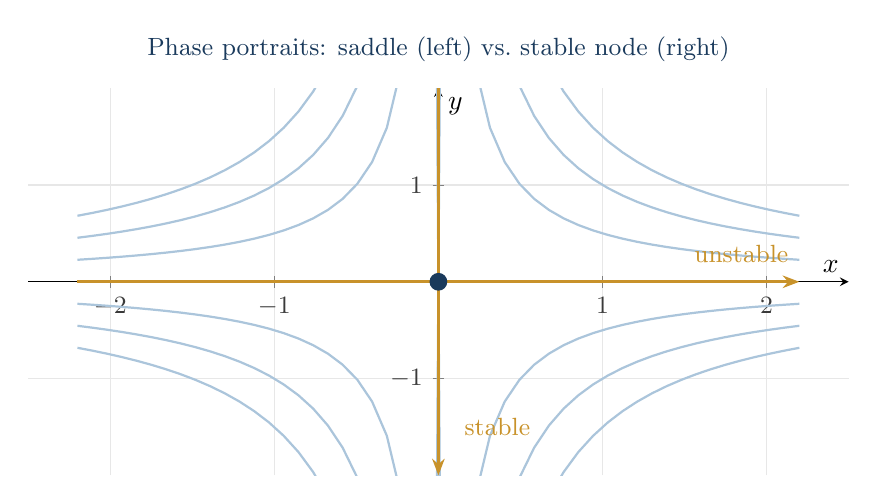
\begin{tikzpicture}
\begin{axis}[
  width=12cm,height=6.5cm,
  axis lines=center,
  xlabel={$x$},ylabel={$y$},
  xmin=-2.5,xmax=2.5,ymin=-2,ymax=2,
  xtick={-2,-1,1,2},ytick={-1,1},
  tick label style={font=\small,color=DarkGrey},
  grid=major,grid style={DarkGrey!12},
  title={\small\color{NavyBlue}Phase portraits: saddle (left) vs.\ stable node (right)},
]
% Saddle: eigenvalues +1 and -1, eigenvectors (1,1) and (1,-1)
% Stable trajectories along (1,-1), unstable along (1,1)
\foreach \c in {0.5,1.0,1.5}{
  \addplot[MidBlue!40,thick,domain=-2.2:2.2,samples=50] {\c/x};
  \addplot[MidBlue!40,thick,domain=-2.2:2.2,samples=50] {-\c/x};
}
\draw[-{Stealth[length=6pt]},Gold,very thick] (axis cs:-2.2,0) -- (axis cs:2.2,0);
\draw[-{Stealth[length=6pt]},Gold,very thick] (axis cs:0,2) -- (axis cs:0,-2);
\node[Gold,font=\small,above right] at (axis cs:1.5,0.1) {unstable};
\node[Gold,font=\small,right] at (axis cs:0.1,-1.5) {stable};
\addplot[only marks,mark=*,mark size=3pt,NavyBlue] coordinates {(0,0)};
\end{axis}
\end{tikzpicture}
\end{center}

\subsection{Step 3: Second-order ODEs as linear algebra}

\begin{problem}
\label{prob:second_order_LA}
The ODE $y'' + by' + cy = 0$ is equivalent to the first-order system $\dot{\mathbf{u}} = A\mathbf{u}$ where $\mathbf{u} = (y,y')^T$ and $A = \begin{pmatrix}0&1\\-c&-b\end{pmatrix}$ (the \textbf{companion matrix}).

\begin{enumerate}[label=(\alph*),topsep=2pt]
  \item Show the characteristic polynomial of $A$ is $\lambda^2+b\lambda+c = 0$ --- exactly the characteristic equation of the ODE from Journey~2. So the ODE and the matrix have the same characteristic polynomial. Is this a coincidence?
  \item Express the harmonic oscillator $\ddot{x}+\omega^2 x=0$ as a $2\times2$ system. Find the eigenvalues of the companion matrix and verify they are $\pm i\omega$.
  \item The phase portrait of the harmonic oscillator in the $(x,\dot{x})$-plane consists of ellipses (or circles if $\omega=1$). Show this follows from the fact that the eigenvalues are purely imaginary.
  \item For the damped oscillator $\ddot{x}+2\gamma\dot{x}+\omega^2 x=0$: the eigenvalues are $-\gamma\pm\sqrt{\gamma^2-\omega^2}$. Express each dynamical regime (underdamped, critically damped, overdamped) as a statement about the phase portrait.
  \item \textbf{Wronskian.} For two solutions $y_1,y_2$ of $y''+py'+qy=0$, the Wronskian is $W = y_1y_2'-y_1'y_2 = \det\begin{pmatrix}y_1&y_2\\y_1'&y_2'\end{pmatrix}$. Prove $W' = -pW$ (Abel's identity), hence $W(x) = W(x_0)e^{-\int p}$. The solutions are linearly independent if and only if $W\neq 0$.
\end{enumerate}
\end{problem}

\subsection{Step 4: Green's functions}

\begin{problem}
\label{prob:greens}
The non-homogeneous problem $Ly = f$ can be solved by the \textbf{Green's function} $G(x,s)$:
\[
  y(x) = \int_a^b G(x,s)f(s)\,ds.
\]
$G(x,s)$ is the response at $x$ due to a unit impulse at $s$.

\begin{enumerate}[label=(\alph*),topsep=2pt]
  \item For $-y'' = f$ on $[0,1]$ with $y(0)=y(1)=0$, the Green's function is $G(x,s) = \begin{cases}x(1-s)&x\leq s\\s(1-x)&x>s\end{cases}$. Verify: (i) $-\partial_x^2 G = 0$ for $x\neq s$; (ii) $G$ satisfies boundary conditions; (iii) $G$ has a jump in $\partial_x G$ of size $-1$ at $x=s$.
  \item Interpret $G(x,s)$ as the deflection at position $x$ of a beam fixed at both ends, under a unit load at $s$. Why is $G$ symmetric: $G(x,s) = G(s,x)$? (What physical principle requires this?)
  \item The Green's function solves $Ly = f$ for \emph{any} $f$ by superposition: write $f = \int f(s)\delta(x-s)\,ds$ (the Dirac delta), apply $L^{-1}$ to get $y = \int G(x,s)f(s)\,ds$. This is the kernel of the inverse operator $L^{-1}$.
  \item Green's function is the matrix of $L^{-1}$ in the ``continuous basis'' $\{\delta(x-s):s\in[0,1]\}$. The symmetry $G(x,s)=G(s,x)$ says $L^{-1}$ is self-adjoint --- which follows because $L$ is self-adjoint. Connect this to the spectral theorem.
  \item Using the Sturm-Liouville spectral expansion (eigenfunctions $\phi_n$ of $L$ with eigenvalues $\lambda_n$): show $G(x,s) = \sum_n\frac{\phi_n(x)\overline{\phi_n(s)}}{\lambda_n}$. This is the spectral expansion of the Green's function.
\end{enumerate}
\end{problem}

\begin{problem}
\label{prob:normal_modes}
\textbf{Normal modes of a coupled oscillator.} Two masses $m$ connected by springs (spring constant $k$ to walls, $\kappa$ between them) satisfy:
\[
  m\ddot{x}_1 = -kx_1 - \kappa(x_1-x_2), \qquad m\ddot{x}_2 = -kx_2 + \kappa(x_1-x_2).
\]

\begin{enumerate}[label=(\alph*),topsep=2pt]
  \item Write as $m\ddot{\mathbf{x}} = -K\mathbf{x}$ for the stiffness matrix $K$. Find $K$.
  \item Try $\mathbf{x}(t)=\mathbf{v}e^{i\omega t}$. Show $\mathbf{v}$ must be an eigenvector of $K$ with eigenvalue $m\omega^2$.
  \item Find the two \textbf{normal mode frequencies} $\omega_1,\omega_2$ and the corresponding mode shapes $\mathbf{v}_1,\mathbf{v}_2$.
  \item The first mode $\mathbf{v}_1=(1,1)/\sqrt{2}$ (in-phase) has frequency $\omega_1=\sqrt{k/m}$. The second mode $\mathbf{v}_2=(1,-1)/\sqrt{2}$ (out-of-phase) has frequency $\omega_2=\sqrt{(k+2\kappa)/m}$. Describe the physical motion of each mode.
  \item Express the general motion as a superposition of normal modes. If the initial condition is $\mathbf{x}(0)=(1,0)$, $\dot{\mathbf{x}}(0)=(0,0)$: write $\mathbf{x}(0)$ as a linear combination of $\mathbf{v}_1$ and $\mathbf{v}_2$, then write $\mathbf{x}(t)$.
\end{enumerate}
\end{problem}

\begin{problem}
\label{prob:variational_ODE}
\textbf{Variation of parameters.} When the homogeneous solution $y_h = c_1y_1+c_2y_2$ is known, the particular solution to $y''+py'+qy=f$ can be found by \emph{varying} the constants $c_1,c_2$ to become functions of $x$.

\begin{enumerate}[label=(\alph*),topsep=2pt]
  \item Assume $y_p = u_1(x)y_1(x) + u_2(x)y_2(x)$ with the constraint $u_1'y_1+u_2'y_2=0$. Substitute into the ODE to derive $u_1'y_1'+u_2'y_2' = f$. Solve for $u_1',u_2'$ using Cramer's rule.
  \item Show the solution is $y_p(x) = \int_a^x\frac{y_1(s)y_2(x)-y_1(x)y_2(s)}{W(s)}f(s)\,ds$ where $W$ is the Wronskian. Identify the Green's function $G(x,s)$.
  \item Apply to solve $y''+y=\sec x$ (note: $y_1=\cos x$, $y_2=\sin x$).
  \item Variation of parameters is the continuous analogue of the change-of-basis formula in linear algebra. Explain this analogy precisely.
\end{enumerate}
\end{problem}

\section{Part 3 \texorpdfstring{---}{--} Discovery}

\begin{discoverybox}
\textbf{The unification of Journey 2 and Journey 3.}

\textbf{First.} The set of solutions to a linear ODE is a vector space of dimension equal to the order. Initial conditions select a specific element --- they are coordinates in the solution space.

\textbf{Second.} Systems $\dot{\mathbf{u}} = A\mathbf{u}$ are solved by eigendecomposition. The eigenvalues of $A$ determine the qualitative behaviour (stability, oscillation); the eigenvectors are the normal modes. Every technique from linear algebra applies directly.

\textbf{Third.} The Green's function is the continuous analogue of a matrix inverse. It encodes the response of a system to any forcing, and its spectral expansion (via eigenfunctions) is the functional calculus of the differential operator.

\textbf{Fourth.} Normal modes of a coupled oscillator, phase portraits of dynamical systems, and Sturm-Liouville eigenfunctions are all instances of one idea: a self-adjoint operator in an inner product space has an orthonormal eigenbasis, and every solution decomposes into a sum of modes.

\medskip
\begin{center}
\renewcommand{\arraystretch}{1.5}
\begin{tabular}{l l l}
\toprule
\textbf{Linear Algebra} & $\longleftrightarrow$ & \textbf{Differential Equations} \\
\midrule
Vector space & $\longleftrightarrow$ & Solution space of $Ly=0$ \\
Linear map $T$ & $\longleftrightarrow$ & Differential operator $L$ \\
Matrix inverse $A^{-1}$ & $\longleftrightarrow$ & Green's function $G(x,s)$ \\
Eigenvalue $\lambda$ & $\longleftrightarrow$ & Characteristic root / resonant frequency \\
Eigenvector $\mathbf{v}$ & $\longleftrightarrow$ & Eigenfunction / normal mode \\
Spectral decomposition & $\longleftrightarrow$ & Normal mode expansion \\
$e^{tA}$ & $\longleftrightarrow$ & Solution operator $e^{tL}$ \\
Jordan block & $\longleftrightarrow$ & Resonance ($te^{\lambda t}$ solutions) \\
\bottomrule
\end{tabular}
\end{center}

\medskip
\textbf{What this means for Journeys 4--7.} Journey~4 (Fields and Space) applies this machinery to vector calculus: the Laplacian, curl, and divergence are linear operators on function spaces, and their eigenvalue problems are the wave equation, heat equation, and Laplace equation. Journey~6 (Fourier/Transforms) is the spectral theory of the differentiation operator applied in full generality.
\end{discoverybox}

\section{Part 4 \texorpdfstring{---}{--} Naming the Ideas}

\begin{namebox}
\textbf{Journey 3 summary.}
\medskip
\begin{center}
\renewcommand{\arraystretch}{1.5}
\begin{tabular}{l l l}
\toprule
\textbf{Module} & \textbf{Core discovery} & \textbf{Key theorem} \\
\midrule
1 & Vector spaces; linear maps; kernel/image & Rank-Nullity \\
2 & Matrices; row reduction; determinants & Four fundamental subspaces \\
3 & Eigenvalues; diagonalisation & Spectral theorem (symmetric) \\
4 & Inner products; SVD & Eckart-Young; Gram-Schmidt \\
5 & Adjoints; functional calculus & Spectral theorem (normal) \\
6 & ODE solution spaces; normal modes & Green's function; Wronskian \\
\bottomrule
\end{tabular}
\end{center}
\end{namebox}

\section{Part 5 \texorpdfstring{---}{--} Deep Problems}

\begin{deepproblem}[The resolvent and the spectrum]
For a linear operator $L$ on a Banach space, the \textbf{resolvent} is $R(\lambda) = (\lambda I - L)^{-1}$ (defined when $\lambda I - L$ is invertible).
\begin{enumerate}[label=(\alph*)]
  \item The \textbf{spectrum} $\sigma(L)$ is the set of $\lambda$ for which $\lambda I - L$ is not invertible. For a finite-dimensional operator this is just the eigenvalues. Show $R(\lambda) - R(\mu) = (\mu-\lambda)R(\lambda)R(\mu)$ (the resolvent identity).
  \item The resolvent is analytic in $\lambda$ away from $\sigma(L)$. Using the resolvent identity, show $\frac{d}{d\lambda}R(\lambda) = -R(\lambda)^2$.
  \item The \textbf{spectral projection} onto the eigenspace for $\lambda_0$ is $P = \frac{1}{2\pi i}\oint_C R(\lambda)\,d\lambda$ (contour integral around $\lambda_0$). For a matrix with distinct eigenvalues, verify this recovers the projection $P_k = \mathbf{v}_k\mathbf{w}_k^T$ (outer product of right and left eigenvectors).
  \item For the Green's function: $G(x,s;\lambda) = $ kernel of $(\lambda I - L)^{-1}$ (the resolvent kernel). Write the spectral expansion of $G$ and explain its poles.
\end{enumerate}
\end{deepproblem}

\begin{deepproblem}[Stability theory and Lyapunov functions]
\begin{enumerate}[label=(\alph*)]
  \item An equilibrium $\mathbf{0}$ of $\dot{\mathbf{u}} = A\mathbf{u}$ is \textbf{asymptotically stable} if all eigenvalues of $A$ have negative real part. Prove that if $A$ is diagonalisable with eigenvalues $\lambda_1,\ldots,\lambda_n$ all satisfying $\text{Re}(\lambda_i) < 0$, then $\|e^{tA}\| \to 0$ as $t\to\infty$.
  \item \textbf{Lyapunov's theorem}: $\mathbf{0}$ is asymptotically stable if and only if for every positive definite $Q$ there exists a positive definite $P$ satisfying $A^TP + PA = -Q$ (the Lyapunov equation). The function $V(\mathbf{u}) = \mathbf{u}^TP\mathbf{u}$ is a \textbf{Lyapunov function}. Show $\dot{V} = -\mathbf{u}^TQ\mathbf{u} < 0$ along trajectories.
  \item For \emph{nonlinear} systems $\dot{\mathbf{u}} = f(\mathbf{u})$, stability is harder. But if $V(\mathbf{u})$ satisfies $V(\mathbf{0})=0$, $V(\mathbf{u})>0$ for $\mathbf{u}\neq\mathbf{0}$, and $\dot{V}=\nabla V\cdot f(\mathbf{u})<0$, then $\mathbf{0}$ is stable. Use $V = x^2+y^2$ to show $\mathbf{0}$ is stable for $\dot{x}=-x^3$, $\dot{y}=-y^3$.
  \item The Lyapunov equation $A^TP+PA=-Q$ is itself a linear equation in $P$. When does it have a unique solution?
\end{enumerate}
\end{deepproblem}

\begin{deepproblem}[Floquet theory: periodic coefficients]
If $A(t+T)=A(t)$ (periodic matrix), the system $\dot{\mathbf{u}}=A(t)\mathbf{u}$ has fundamentally different structure from the constant-coefficient case.
\begin{enumerate}[label=(\alph*)]
  \item Define the \textbf{monodromy matrix} $M = \Phi(T)$ where $\Phi(t)$ is the fundamental matrix solution ($\dot\Phi=A\Phi$, $\Phi(0)=I$). Show solutions are related over one period by $\mathbf{u}(t+T) = M\mathbf{u}(t)$.
  \item \textbf{Floquet's theorem}: $\Phi(t) = P(t)e^{Bt}$ where $P(t+T)=P(t)$ is periodic and $B$ is a constant matrix with $e^{BT}=M$. The eigenvalues of $B$ are the \textbf{Floquet exponents}; those of $M$ are the \textbf{Floquet multipliers}.
  \item Stability is governed by the Floquet multipliers: the system is stable if all multipliers satisfy $|\mu_i|\leq 1$. Explain why this is the analogue of ``eigenvalues have negative real part'' for constant-coefficient systems.
  \item \textbf{Mathieu's equation}: $\ddot{x}+(a-2q\cos 2t)x=0$ (pendulum with vibrating support). The stability boundaries in the $(a,q)$-parameter plane form the \textbf{Mathieu stability diagram}. Describe qualitatively: for which parameters is the pendulum stable?
\end{enumerate}
\end{deepproblem}

\section{Part 6 \texorpdfstring{---}{--} Reflection}

\begin{reflectionbox}
\textbf{Final reflection for Journey 3.}

\begin{enumerate}
  \item \textbf{On the dictionary.} This module presented a dictionary between linear algebra and differential equations. Every concept in one language has a translation in the other. Does building a dictionary feel like discovering that two things are the same, or like discovering a useful analogy between two different things? Is there a meaningful distinction?

  \item \textbf{On normal modes.} The coupled oscillator's motion decomposes into normal modes that evolve independently. In quantum mechanics, the same decomposition into energy eigenstates describes any quantum system. In signal processing, the Fourier decomposition is the normal mode expansion of the differentiation operator. Write a paragraph: why does the concept of ``decompose into independent modes'' appear in so many different physical contexts?

  \item \textbf{On Green's functions.} The Green's function is the inverse of a differential operator written as a kernel. The spectral expansion of the Green's function involves the eigenfunctions of the operator. Write down the chain of ideas from ``$A^{-1}$'' (matrix inverse) to ``$G(x,s)$'' (Green's function) explicitly: what changes, what stays the same?

  \item \textbf{Looking ahead.} Journey~4 (Fields and Space) applies these ideas to vector-valued functions in three dimensions: the gradient, divergence, and curl are linear operators; the wave equation, heat equation, and Laplace equation are their eigenvalue problems; Green's functions in three dimensions are the fundamental solutions of electrostatics and gravity. Name one specific physical problem from Journey~4 that you anticipate will require the tools of both Journey~2 and Journey~3.
\end{enumerate}
\end{reflectionbox}

\vspace{0.8cm}
\begin{namebox}
\textbf{What Journey 3 built --- and where it feeds.}

\medskip
Journey~3 built the language of linearity in full generality: from the abstract axioms of a vector space through to the spectral theory of operators on Hilbert spaces. Every subsequent journey uses this language.

Journey~4 uses linear maps on $\mathbb{R}^3$ (gradient, divergence, curl) and the eigenvalue theory of the Laplacian.

Journey~5 (Probability) uses linear maps on function spaces (expectation, variance) and the spectral theory of Markov operators.

Journey~6 (Fourier/Transforms) is the spectral theory of the differentiation operator: the Fourier transform diagonalises $d/dx$, just as eigenvectors diagonalise a matrix.

Journey~7 (Abstraction) treats all of this as special cases of category theory and algebraic structures.

\medskip
You are not finished with linear algebra. You are in the middle of it.
\end{namebox}

\vspace{1cm}
\begin{center}
{\color{Gold}\rule{0.6\linewidth}{1.2pt}}\\[8pt]
{\large\bfseries\color{NavyBlue}End of Journey 3: Linear Structure}\\[6pt]
{\normalsize\color{DarkGrey}\itshape Six modules. Vector spaces, matrices, eigenvalues, inner products, adjoints, and the bridge to differential equations.}\\[10pt]
{\color{Gold}\rule{0.6\linewidth}{1.2pt}}\\[10pt]
{\small\color{DarkGrey}Continue to: \textbf{Journey 4 --- Fields and Space}}\\[4pt]
{\small\color{DarkGrey}\itshape ``The purpose of abstraction is not to be vague,\\but to create a new semantic level in which one can be absolutely precise.''\\
\upshape --- Edsger Dijkstra}
\end{center}

\end{document}